\chapter{Physical cluster provisioner}
\label{sec:remotevirt}

A resource provisioner is an entity able to provision resources in the form of \gls{slurm} daemons upon request by the \gls{vurm} controller. The \gls{vurm} architecture allows multiple, stackable, resource provisioners and comes with two different implementations. One of them, the physical cluster provisioner, is further described in this chapter.

For additional information about the exact role of a resource provisioner, how it fits into the \gls{vurm} architecture and which tasks it has to be able to accomplish, refer to the \emph{\nameref{sec:architecture}} chapter at page \pageref{sec:architecture}.

The physical cluster provisioner is conceived to manage Linux based HPC clusters. This provisioner is able to execute \gls{slurm} daemons on virtual machines spawned on physical nodes of the cluster and feed them to the \gls{slurm} controller. Additionally this module is also responsible to manage virtual machine migration between physical nodes to better exploit the available computational resources.

The different aspects covered by this chapter are structured as follows:

\begin{itemize}
    \item Section \ref{sec:cluster-arch} aims to describe the provisioner specific architecture, including description of both internal and external software components, networking configuration and system deployment;
    \item Section \ref{sec:libvirt-integration} introduces some \texttt{libvirt} related concepts and describes the \gls{xml} domain description file used to configure the guests;
    \item Section \ref{sec:vm-lifecycle} deals with different aspects of the virtual machine lifecycle, such as setup, \gls{ip} address retrieval or public key exchange.
\end{itemize}

Aspects directly bound to \gls{vm} migration between physical nodes will not be discussed in this chapter. Refer to the \emph{\nameref{sec:migration}} chapter, starting at page \pageref{sec:migration}, for additional information about this topic.


\section{Architecture}
\label{sec:cluster-arch}

* Need for a central controller and distributed daemons

\subsection{Components}

* Describe the components

\subsection{Deployment}

* Introduce the deployment diagram, define the relationships

\begin{todo}
Design and describe the complete system deployment diagram (provisioner, manager, libvirtd, physical and virtual nodes).
\end{todo}


\section{Libvirt integration}
\label{sec:libvirt-integration}

\subsection{Naming conventions}

\begin{todo}
Especially mention domains vs. node vs. hypervisor.
\end{todo}

\subsection{XML Description file}


\section{VM Lifecycle}
\label{sec:vm-lifecycle}

\begin{todo}
Design and describe a sequence diagram illustrating the whole VM lifecycle and use it in the different sections below. The provisioner shall be an actor while the remote node manager one of the main components.
\end{todo}

\subsection{Volumes cloning}

During the virtual cluster creation phase, the user has the possibility to choose which disk image all the created VMs will be booted from.

As a virtual cluster is formed by multiple VMs, and as each virtual machine needs its own disk image which read from and write to, multiple copies of the base image have to be created.

Performing a raw copy of the base image presents obvious limitations: firstly each copy occupies the same amount of space as the original image, which rapidly leads to fill up the available space on the storage support, and secondly, given the necessity of these images to live on a shared file system (see section XX for the details), the copy operation can easily fill up the available network bandwidth and take a significant amount of time.

\begin{todo}
Reference to the migration chapter where the KVM requirements for the live migration are presented (all disk images have to live on a shared storage).
\end{todo}

To overcome these drawbacks, a particular disk image format called \texttt{QCOW2} (Qemu Copy On Write, version 2) is used. This particular format has two useful features:

\begin{itemize}
    \item A \texttt{qcow2} image file, unlike a \texttt{raw} disk image, occupies only the equivalent of the size of the data effectively written to the disk. This means that it is possible to create a 40GB disk image which, once a base OS is installed on it, occupies only a couple of GBs\footnote{Other disk image formats support this feature too. For example \texttt{qcow} (version 1) or \texttt{VMDK} (when using the \texttt{sparse} option).}.
    \item It is possible to create a disk image based on another one. Read data is retrieved from the base image until the guest modifies it. Modified data is written only to the new image, while leaving the base image intact. The figure X represents this process graphically.
\end{itemize}

\begin{todo}
Reference image correctly.
\end{todo}

\begin{figure}[h]
	\centering
	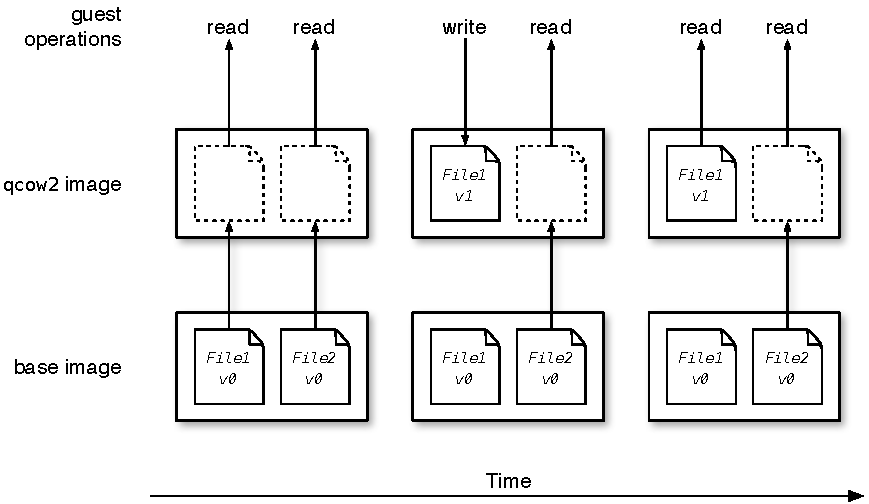
\includegraphics[width=0.6\textwidth]{figures/cow-images}
	\caption{Copy-On-Write image R/W streams}
	\label{fig:cow}
\end{figure}

The combination of these two features allows to create per-VM disk images in both a time- and space-efficient manner.

\subsection{IP address retrieval}

The simplest way to interact with a newly started guest is through a TCP/IP connection. The vurm tools use \texttt{ssh} to execute commands on the guest, while the slurm controller communicates with its daemons over a socket connection. All of these communications means require the IP address (or the hostname) of the guest to be known.

At present, libvirt does not exposes any APIs to retrieve a guests IP address and a solution to overcome this shortcoming has to be implemented completely by the calling codebase.

During the execution of the project, different methods were analyzed and compared; the rest of this sub section is dedicated to analyze the advantages and shortcomings of each of them.


\subsubsection{Inspect host-local ARP tables}

As soon as a guest establish a TCP connection with the outside world, it has to advertise its IP address in an ARP response. This causes the host to pick it up and cache it its ARP table.

Running the \texttt{arp -an} command on the host will reveal the contents of the ARP table, as presented in listing Z:

\lstset{language=bash,caption=Example \texttt{arp -an} output,label=lst:arp}
\begin{lstlisting}
$ arp -an
? (10.0.0.1) at 0:30:48:c6:35:ea on en0 ifscope [ethernet]
? (10.0.0.95) at 52:54:0:48:5c:1f on en0 ifscope [ethernet]
? (10.0.1.101) at 0:14:4f:2:59:ae on en0 ifscope [ethernet]
? (10.0.6.30) at 52:54:56:0:0:1 on en0 ifscope [ethernet]
? (10.255.255.255) at ff:ff:ff:ff:ff:ff on en0 ifscope [ethernet]
? (129.24.176.1) at 0:1c:e:f:7c:0 on en1 ifscope [ethernet]
? (129.24.183.255) at ff:ff:ff:ff:ff:ff on en1 ifscope [ethernet]
? (169.254.255.255) at (incomplete) on en0 [ethernet]
\end{lstlisting}

As libvirt is able to retrieve the MAC address associated with a given interface, it is possible to parse the output and retrieve the correct IP address.

This method could not be adopted because ARP packets do not pass across routed newtorks and the bridged network layout would thus stop them.


\subsubsection{Proprietary VM Tools}

Some hypervisors (as, for example, VMWare ESXi or VirtualBox), are coupled with a piece of software which can be installed on the target guest and provides additional interaction capabilities, such as commands execution, enhanced virtual drivers or, in this case, IP address retrieval.

Such a tool would bind the whole system to a single hypervisor and would vanish the efforts done to support the complete range of libvirt-compatible virtual machine monitors. Additionally, the KVM/Qemu pair, chosen for their live migration support, do not provide such a tool.


\subsubsection{Static DHCP entries}

A second possible method is to configure a pool of statically defined IP/MAC address couples in the DHCP server and configure the MAC address in the libvirt XML domain description file in order to be sure of which IP address would be assigned to the VM.

This method could have worked and is a viable alternative; it was however preferred to not depend on external services (the DHCP server, in this case) and provide a solution which can work in every context.

A configuration switch to provide a list of IP/MAC address pairs instead of te adopted solution can although be considered as a future improvement.


\subsubsection{Serial to TCP data exchange}

The last explored and successfully adopted method takes advantage of the serial port emulation feature provided by the different hypervisors and the capability to bind them to (or connect them with) a TCP endpoint of choice.

In the actual implementation, the VURM daemon listens on a new (random) port before it spawns a new VM; the libvirt daemon will then provide a serial port to the guest and connect it to the listening server. Once booted, a little script on the guest writes the IP address to the serial port and the TCP server receives it as a normal TCP/IP data stream.

Although not authenticated nor encrypted, this communication channel is deemed secure enough as no other entity can possibly obtain relevant information by eavesdropping the communication (only an IP address is exchanged). Additionally, as it's the hypervisor task to establish the TCP connection directly to the local host, there is no danger for man-in-the-middle attacks (and thus invalid information being transmitted).\footnote{The daemon only binds to the loopback interface; a malicious process should be running on the same host to possibly connect to the socket and send a wrong IP address}
The code snippet XY contains the needed libvirt device configuration:

\lstset{language=xml,caption=Libvirt TCP to serial port device description,label=lst:serialtcp}
\begin{lstlisting}
<serial type="tcp">
    <source mode="connect" host="127.0.0.1" service="$PORT"/>
    <protocol type="raw"/>
    <target port="1"/>
    <alias name="serial0"/>
</serial>
\end{lstlisting}

The shell script on the guest needed to write the IP address to the serial device can be as simple as the following:

\lstset{language=bash,caption=Shell script to write the IP address to the serial port,label=lst:serialip}
\begin{lstlisting}
#!/bin/sh
ifconfig eth0 | grep -oE '([0-9]{1,3}\.){3}[0-9]{1,3}' | head -1 >/dev/ttyS0
\end{lstlisting}

The actual implementation is more complex and accounts for the public key exchange part too (see section XY).


\begin{todo}
Refer to the sequence diagram (actually, it may be useful to draw it before).
Rephrase the description, maybe with more references to the diagram.
Reference sections.
Implement simple VM tools?
\end{todo}


\subsection{Public key exchange}

As anticipated in section XZ, the VURM daemon executes command on the guest through a SSH connection. The daemon authentication modes were deliberately restricted, for security reasons, to public key authentication only.

This restriction requires that the daemon public key is correctly installed on the guest disk image. As the disk image is customizable by the user, it is necessary to define how this public key will be installed.

Different techniques can be used to achieve this result; the rest of this subsection is dedicated to analyze three of them.

\subsubsection{Public key as a requirement}

The simplest (from the VURM point of view) solution is to set the setup of a VURM-specific user account with a given public key a requirement to run a custom disk image on a given VURM deployment.

This approach requires the end user to manually configure its custom disk image. The obvious drawback is the inability to run the same disk image on different VURM deployments as the key pair differs from setup to setup.\footnote{This is, however, a very minor drawback; the percentual of users running jobs on different clusters is very low, and even so, the disk image probably needs adjustments of other parameters anyway.}

The final chosen solution is based on this approach, given that the disk image has to be specifically customized because of other parameters anyway (refer to Appendix Z).

\subsubsection{Pre-boot key installation}

Another explored technique consisted of mounting the disk image on the host, copying the public key to the correct location, unmounting the image and then starting the guest.

The mounting, copying and unmounting operation was made straightforward by the use of a specific image manipulation library called \texttt{libguestfs}.

For security reasons, this library would spawn a new especially crafted VM instead of mounting the image directly on the host; this made the whole key installation operation long task when compared with the simplicity of the problem (mounting, copying and unmouting took an average of 5 seconds during the preliminary tests).

The poor performances of the operation, its different dependencies (too many for such a simple operation) and its tight coupling with the final public key path on the guest, led this approach to be discarded in the early prototyping phase.

\subsubsection{IP-Key exchange}

As seen in the previous section, the final solution adopted to retrieve a guest IP address, already requires to setup a communication channel between the VURM daemon and the guest.

The idea of this approach is to send back the public key to the guest as soon as the IP address is received. In this case, the guest would first write the IP address to the serial port and then read the public key and store it to the appropriate location. An extension to the shell script XZ which saves the public key as a valid key to login as root is presented in the listing XY:

\lstset{language=bash,caption=Shell script to write the IP address to the serial port,label=lst:serialip}
\begin{lstlisting}
#!/bin/sh
ifconfig eth0 | grep -oE '([0-9]{1,3}\.){3}[0-9]{1,3}' | head -1 >/dev/ttyS0
mkdir -p /root/.ssh
chmod 0755 /root/.ssh
cat /dev/sttyS0 >>/root/.ssh/authorized_keys
chmod 0644 /root/.ssh/authorized_keys
\end{lstlisting}

This technique was firstly adopted, but then discarded in favor of the more proper requirement-based solution as bidirectional communication using a serial port revealed to be too complicated to implement correctly in a simple shell script.\footnote{Synchronization and timing issues which could not simply be solved by using timeouts where detected when running slow guests.}

A proper solution would have required the installation of a custom built utility; copying a simple file (the public key) was considered a less troublesome operation than installing yet another utility along with its dependencies.


\begin{todo}
Refer to the right appendix and write it (disk image creation guide).
\end{todo}


\section{Future developments}

\subsection{Disk image transfer}

\subsection{Support for alternative VLAN setups}
